\documentclass[10pt,twocolumn]{article}
\usepackage[margin=0.72in]{geometry}
\usepackage[T1]{fontenc}
\usepackage{lmodern,amsmath,amssymb,booktabs,graphicx,hyperref,microtype,longtable}
\hypersetup{colorlinks=true,urlcolor=blue,linkcolor=blue}
\newcommand{\EpisodeCount}{69}
\newcommand{\ProbeCount}{196}
\newcommand{\PairCount}{59}
\newcommand{\SourceCount}{5}
\newcommand{\ProfileCount}{6}
\newcommand{\OracleCount}{35}
\newcommand{\ProductCount}{1,420,363}
\newcommand{\EdgeCount}{11,230,303}
\newcommand{\MaxGap}{18}
\newcommand{\OldLabels}{1,802,728}

\title{BrickPlan 2.0: Certified Resource and Inspection\\Planning with Visual Assembly Observations}
\author{Benchmark research release}
\date{October 8, 2026}
\begin{document}
\raggedbottom
\maketitle

\begin{abstract}
Long assembly sequences need not require substantial planning. An exhaustive
audit of our preceding benchmark finds that a static blocker-closure formula
exactly recovers all \OldLabels{} stored state--goal costs. We redesign the
task around a finite external rack and persistent off-assembly inspection
obligations, while retaining original source poses and qualified insertion
paths. The resulting bank contains \EpisodeCount{} interactive episodes,
\ProbeCount{} diagnostic responses and \PairCount{} matched pairs across
\ProfileCount{} profiles from \SourceCount{} source kits.
Directed exact oracles certify every retained product state and transition.
The static closure bound now underestimates completion cost by up to
\MaxGap{} operations; identical assemblies can require disjoint optimal
next actions when their visible inspection ledgers differ.
Across 207 repeated task-runs, closure greedy completes 189 but is optimal
in only 91; capacity-aware dispatch completes 170, and closure A* with
100 expansions completes 162. Full closure A* solves every task optimally
with at most 2,555 expansions. This is evidence of nontrivial resource
scheduling under a declared abstraction, not general computational hardness.
We provide matched image and structured interfaces, conditional-cost and
recovery metrics, authoritative transcript replay, and budget-accounted
external-policy collection. VLM and human experiments remain unmeasured.
\end{abstract}

\section{Introduction}
A benchmark can contain visually complex objects, long solutions and many
temporary removals while still admitting a short analytic rule. Such a
benchmark may test relation extraction, but its solution length alone does
not establish a planning challenge. BrickPlan 2.0 begins with an explicit
falsification of the earlier difficulty claim and a mechanism-level repair.

Consider a technician who must restore an assembly and inspect selected
parts outside it. A removed part occupies a rack holder. If the rack is
full, another piece may have to be installed temporarily before a necessary
removal is possible. Inspection persists after reattachment: two visually
identical assemblies can have different unfinished obligations. The final
shape, current occupancy and static access relations no longer determine
the complete mission state.

Our contribution is an executable diagnostic contract: a new resource and
inspection state space with exact labels, paired tests that isolate
intermediate order and mission history, and metrics separating immediate
illegality from added future cost and delayed recovery. We make the
selection process and simple-control performance explicit. Neither large
scene size nor a failed weak baseline substitutes for this evidence.

\paragraph{Relation to prior assembly work.}
Break and Make introduces interactive disassembly and reconstruction in
LTRON~\cite{ltron}. InstructioNet builds an explicit visual instruction memory
to support reconstruction~\cite{instructionet}. These works already establish
interactive structural understanding and long assembly sequences.
BrickPlan uses a narrower known-site action space to obtain exact
counterfactual costs and event-level error labels. Our visible inspection
ledger is a declared task variable, not a claim of latent episodic memory.
Resource limits, shortest-path search and admissible heuristics are
established planning tools~\cite{astar}; our contribution is their audited
integration with source-qualified visual assembly diagnostics.

\section{Experimental design and reporting contract}
\label{sec:design}
\begin{table}[t]
\centering\small
\caption{Planned empirical slots. No row has measured results. Exact
model versions, providers and participant cohorts must be registered
before collection.}
\begin{tabular}{p{.55\columnwidth}p{.32\columnwidth}}\toprule
Condition & Measurement status\\\midrule
VLM, image+ID, stepwise actions & Not evaluated\\
Same VLM, image+ID, explicit plan & Not evaluated\\
Same VLM, structured input & Not evaluated\\
Human, image+ID & Not evaluated\\
Human, structured input & Not evaluated\\\bottomrule
\end{tabular}
\end{table}
All conditions share task assignments, identity seeds, operation limits and
camera options. Each manifest records participant/model identity, condition,
version, prompt and configuration hashes, provider, temperature, reasoning
setting, input/output limits, request cap and accounting mode.
We recommend an initial format-and-cost pilot followed by preregistered
collection; the release does not report simulated human or VLM scores.

Primary outcomes are completion over all assigned episodes, optimal
completion, successful regret with coverage, and conditional cost added
over all observed decisions. Diagnostic outcomes cover next-action choice,
continuation failure localization, paired consistency, diagnosis and
recovery. Software search sees the private relation graph and is reported
separately from both public tracks.

Roadster and kart share kit 31027. Development groups are 31027 and 31028;
10156, 31009 and 5867 carry held-out-source labels. The generator has used
all five groups' geometry and solver results to select challenge instances.
This is therefore a public challenge partition, not a blind held-out test.
Seeds permute identities and tie orders; they do not create independent
structures. Results require source-group summaries and explicit missing
assignments. Five groups do not support strong population-level claims.

\section{Why the preceding bank was simple}
\label{sec:audit}
Let $s$ and $g$ be sets of installed registered sites. Initialize a removal
set with occupied unwanted sites and occupied blockers of missing target
sites. Repeatedly add occupied blockers of every site already in that set,
obtaining $R(s,g)$. The static quantity
\begin{equation}
h_{\mathrm{old}}(s,g)=|s\triangle g|+2|R(s,g)\cap g|
\label{eq:old}
\end{equation}
counts required occupancy changes and detach--reattach pairs for occupied
target pieces that must be removed.

An exhaustive audit compares this formula with all reachable labels in
every stored goal table of version 1.2: 70,060 roadster labels, 312,228 kart
labels and 1,420,440 airframe labels. Every comparison is equal.
Computing Eq.~\ref{eq:old} needs static relations but no state-space search
or cost table. This is a finite-bank equality result, not a theorem for all
assembly geometries. It is stronger than observing that a rule solves the
15 selected episodes.

Unlimited temporary storage permitted an all-removals-then-attachments
strategy. Occupancy encoded the entire state; no completed work survived
outside that encoding. Supplied-plan failure localization could measure
execution checking without measuring action selection. Hamming-only
lookahead controls substantially understated what static relations could
already provide. These are task-design issues rather than an insufficient
number of distractors.

\section{Certified workcell and mission state}
\label{sec:mission}
\subsection{Source-qualified physical transitions}
Each registered physical piece $P_i$ fits one original source site $S_i$;
even identical part types are not interchangeable in this protocol.
Unregistered fixed parts form one stud-connected clamped subassembly.
Every installed piece must remain stud-connected to it. Attach/detach
operations follow a qualified straight translation at the original source
orientation, with current blockers and endpoint connectivity determining
legality. No goal or future-cost table participates in execution.

The geometry qualification uses closed collision proxies, a 0.25 LDU
surface inset and a 0.002 LDU guard inherited from the predecessor.
Endpoint tests and continuous straight-path tests reject intersections
or unresolved geometry. Interval clearance uses a translation-distance
bound; the source display meshes remain original LDraw triangles.
The qualification is numerical evidence within this proxy/path model,
not measured contact mechanics.

We retain the three earlier profiles and qualify truck, cottage roof and
sports-car profiles without changing source transforms. A pizza-shop
candidate fails endpoint qualification and is excluded. Larger scenes do
not automatically supply more movable sites: the cottage profile has
18 registered sites but only 17 move in its full-assembly component;
the sports-car profile has 22 registered sites but only 10 move.
The latter remains an easy control.

\begin{table*}[t]
\centering\small
\caption{Source census. ``Parts'' counts the retained source subassembly,
not necessarily the complete source kit. ``Move'' counts registered sites
that can move in the full-assembly component with unlimited rack capacity.
``Rack'' is the finite challenge capacity; D1 controls may use a larger rack.}
\begin{tabular}{llrrrrrr}\toprule
Profile & Kit & Parts & Reg. & Move & Rack & Episodes & Max gap\\\midrule
Roadster body & 31027 & 37 & 17 & 17 & 9 & 14 & 18\\
Kart deck & 31027 & 25 & 18 & 18 & 5 & 14 & 10\\
Airframe & 31028 & 24 & 21 & 21 & 8 & 14 & 4\\
Truck cab and roof & 10156 & 76 & 18 & 18 & 12 & 10 & 6\\
House roof assembly & 31009 & 221 & 18 & 17 & 5 & 14 & 4\\
Sports car upper body & 5867 & 149 & 22 & 10 & 8 & 3 & 0\\
\bottomrule\end{tabular}

\label{tab:sources}
\end{table*}

\subsection{Finite rack and persistent work orders}
Let the full mission state be $x=(s,z)$, where $z$ is the set of completed
inspection jobs. The mission specifies target $g$, rack capacity $K$, and
declared job set $J$. Every detached registered piece occupies one
universal oversized holder:
\[
q(s)=n-|s|\leq K.
\]
A legal detach must preserve this inequality. An \texttt{audit} of $i$
is legal exactly when $i\in J\setminus z$ and $i\notin s$; it changes
$z$ to $z\cup\{i\}$. Completion requires $(s,z)=(g,J)$ and an explicit
\texttt{finish}. The ledger is visible and persists after reattachment.
An eligible audit never competes for a hidden resource or outcome.

Each structural attempt or audit attempt costs one operation, including
rejections. Valid camera acquisitions, diagnoses and finish cost zero.
Budgets depend only on visible size: $6n+2|J|$ operation attempts,
12 additional views and 12 diagnoses. Spending the final operation
without finishing terminates by budget. Detached-piece transfers to rack
holders are abstracted; we do not certify a physical rack layout or hand
trajectory. Executable installed states retain the source poses.

\subsection{Exact costs and a strong static bound}
We compress the reachable physical component to an indexed graph and take
its product with the $2^{|J|}$ inspection flags. Goal-rooted reverse BFS
handles physical edges in both directions; a reverse audit clears a flag
only at a state where its piece is detached.
Let $C^*(x)$ be exact remaining operations. Every table is exhaustively
checked for terminal labels, Bellman equality, runtime-edge agreement,
physical inverses and the lower bound below. The \OracleCount{} retained
tables contain \ProductCount{} state entries and \EdgeCount{} directed
transition entries. These totals include repeated physical states under
different missions; they are not independent examples.

Extend $R$ to include all occupied unfinished inspection pieces before
taking occupied-blocker closure. A resource-relaxed bound is
\begin{equation}
h(x)=|s\triangle g|+2|R(x)\cap g|+|J\setminus z|.
\label{eq:bound}
\end{equation}
It counts unavoidable operations while dropping rack and support scheduling
constraints. Every retained label satisfies $h(x)\leq C^*(x)$.
The gap $C^*(x)-h(x)$ reaches 18. For the roadster task in
Fig.~\ref{fig:replay}, the start has nine rack occupants, the bound is 24
and the optimum is 42; its unique optimal first operation is an attachment.
This supplies a direct counterexample to reusing the old exact-cost formula.

\begin{figure*}[t]
\centering
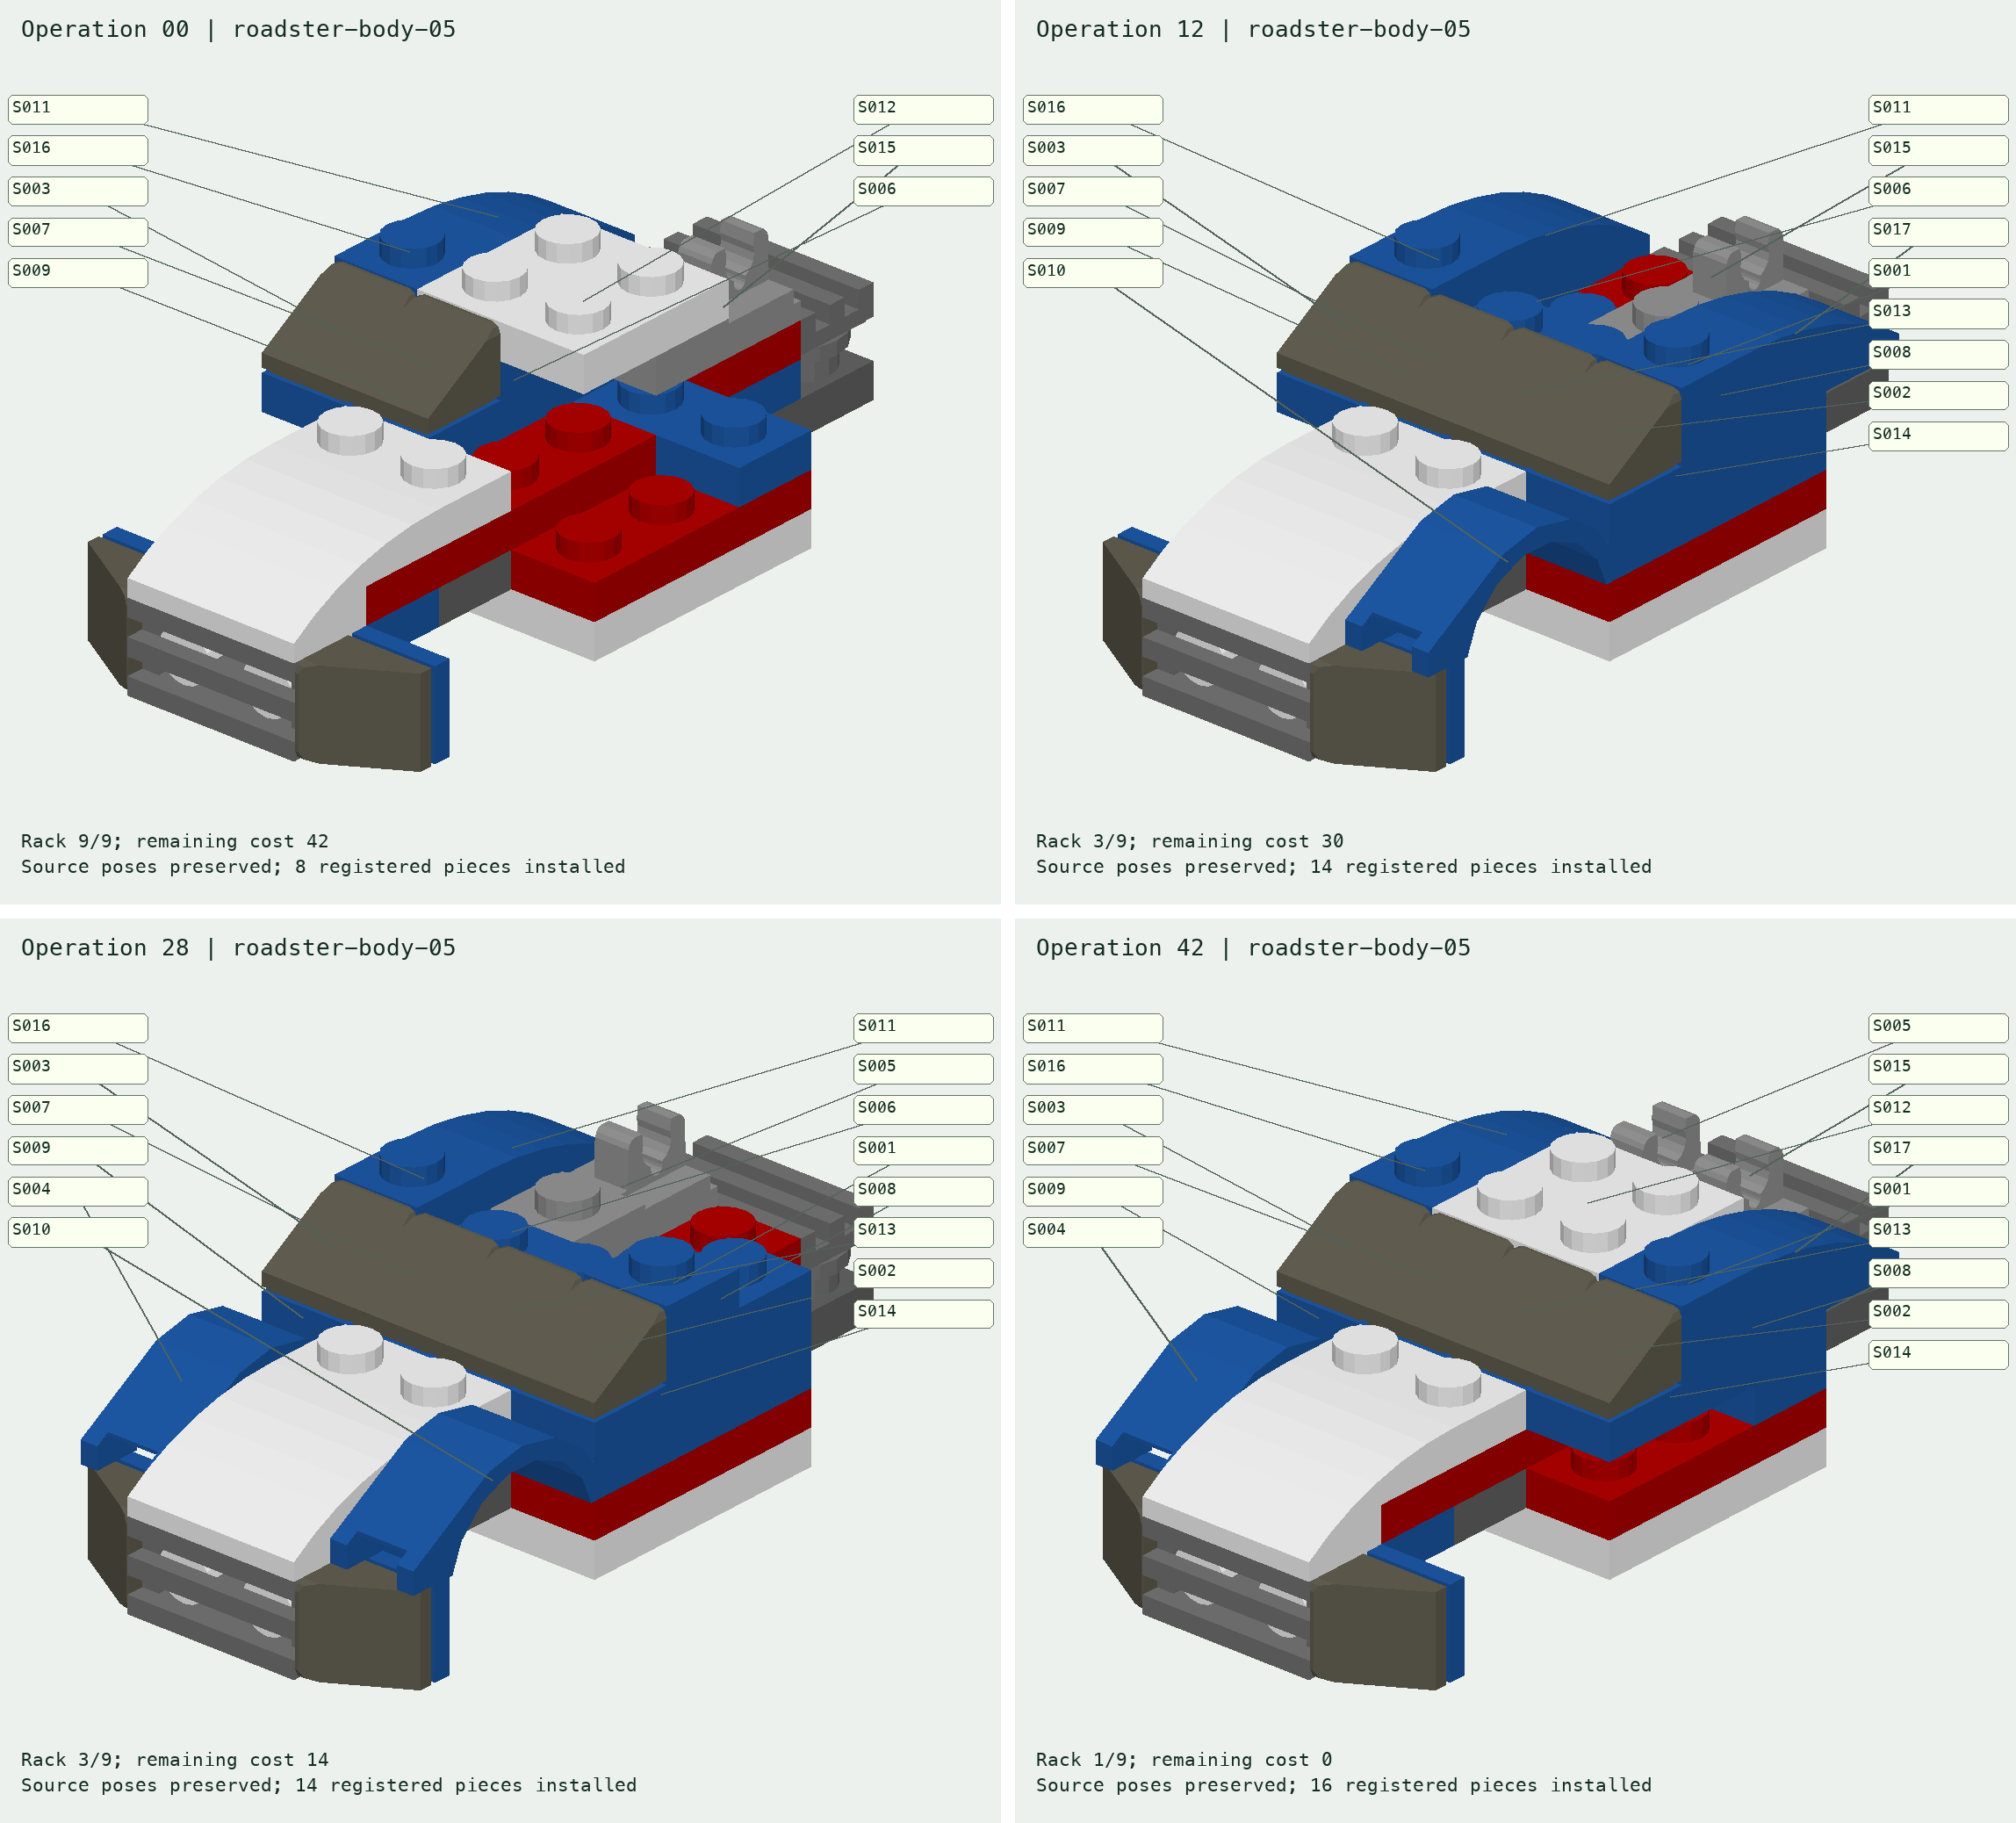
\includegraphics[width=.95\textwidth]{figures/resource-replay.png}
\caption{Authoritative replay of roadster-body-05, identity seed 31.
All four assemblies retain source poses and stud connectivity.
The finite rack requires temporary installation and repeated access
restoration: $h=24$ versus $C^*=42$. Labels identify source sites.
Detached pieces occupy the external rack abstraction and are not depicted
as suspended installed pieces. Frame states and image hashes are supplied.}
\label{fig:replay}
\end{figure*}

\section{Challenge construction and matched diagnostics}
\begin{table}[t]
\centering\small
\caption{Operational tiers. A* counts use the closure heuristic and seed 0.
Tiers encode mechanisms, not a universal monotone hardness ranking.}
\begin{tabular}{lrrrr}\toprule
Tier & Episodes & $C^*$ range & Gap range & A* max\\\midrule
D1 & 13 & 10--33 & 0--0 & 33\\
D2 & 16 & 16--42 & 2--18 & 2555\\
D3 & 34 & 9--40 & 0--10 & 2185\\
D4 & 6 & 33--42 & 6--10 & 2131\\
\bottomrule\end{tabular}

\label{tab:tiers}
\end{table}
D1 retains unlimited-rack and measured easy inspection controls.
D2 selects finite-rack reconfiguration with gap at least two.
D3 includes inspection/resource missions and certified history or changed-work
contrasts; paired members need not individually have a positive gap.
D4 requires at least two jobs, gap at least four and more than 100 closure-A*
expansions under seed 0. Instances are selected from exact rankings with
start-state diversity constraints. These labels are explicitly conditioned
on the chosen mechanism and algorithm. Some D2 instances require more
expansions than D4 instances.

The bank has 98 next-action and 98 continuation responses. Next-action
checkpoints include legal actions that differ in exact conditional cost.
Every cost-minimizing offered action receives credit, including ties.
Forty-nine continuation pairs preserve the initial state, first and last
operations, length and action multiset. Swapping interior operations
creates the contrast between a legal plan and its first execution conflict.
A classifier restricted to the invariant features cannot correctly label
both members: its response accuracy is at most 50\%, and its joint pair
accuracy is zero. The release tests this particular shortcut, not all
possible shortcuts or balanced failure positions.

Five history pairs share assembly, physical target and work-order set but
differ in completed flags. Five future-work pairs share assembly and
physical target but change the requested inspection piece.
Each pair has disjoint optimal initial action sets, and neither set contains
an audit. This avoids reducing the contrast to ``audit the only available
job.'' The changed information is public; hidden memory is not required.
These ten pairs are episode pairs; the other 49 are diagnostic pairs.

\begin{figure*}[t]
\centering
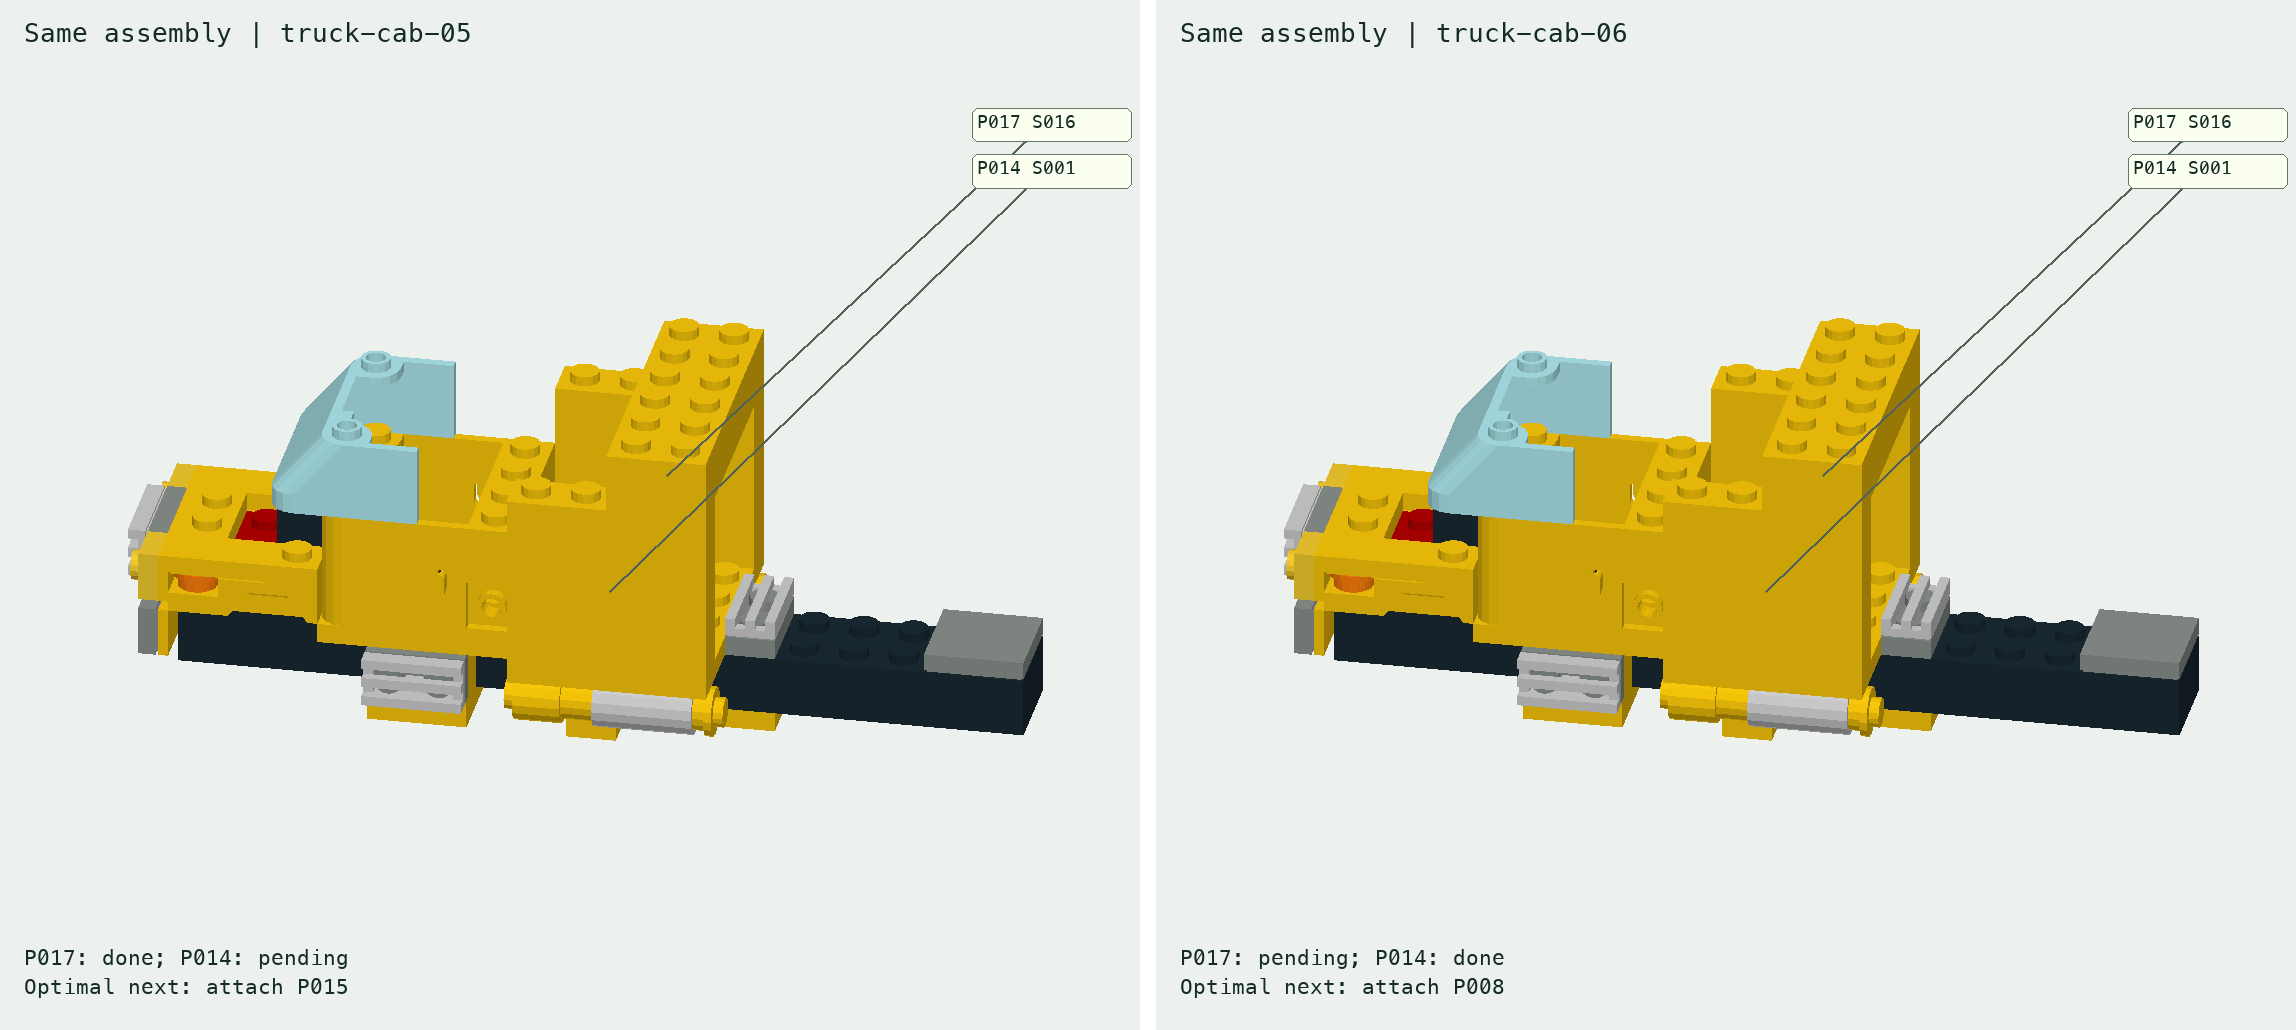
\includegraphics[width=\textwidth]{figures/ledger-contrast.png}
\caption{Truck history pair with identical assembly occupancy and different
visible completion ledgers. The certified optimal next-action sets are
disjoint. Figure labels expose evaluator answers for explanation; study
observations omit those answers. All P/S identifiers follow seed 31.}
\label{fig:history}
\end{figure*}

\section{Visual observations and collection}
The image+ID track supplies five PNG panels: current assembly, target,
all-site reference, registered-piece catalog and occupied rack.
Public text includes registered P/S mapping, rack counts, work orders and
budgets. It excludes source matrices, installed-site flags, blocker/support
graphs, legal-action lists, depth buffers, costs, tiers and pair identities.
The catalog and fixed registration deliberately simplify correspondence.
Rack pixels also expose which physical pieces are outside the assembly.
This track still requires interpreting shape and access, but is not a
test of wholly implicit object identity.

The structured track adds matrices, types, colors, paths and occupancy.
It also includes the same rasters, without the private relation graph.
Humans and agents use the same seven fixed cameras and exploded reference
option. Explosion changes only the reference diagram, never executable
current or target states. Each acquired view is saved at its revision;
revisiting stored pixels is free and does not change executable state.
Free 3D orbit, zoom and explosion are available only after a practice
episode ends.

The local server fixes condition, seed, assignments and run identity.
Study starts are single-use and probe answers freeze on first acceptance.
Revisioned requests are idempotent across restart; persistence is atomic
with in-memory rollback on failure. Administrative collection replays
every episode and probe request and rejects mismatched identities,
answers and view histories. Missing assignments remain in the census.
Static routes form an allowlist; private bank, geometry and cost files
are not served in study mode.

The external adapter consumes public JSON and must pass every raster to
the provider as an image, including retained views. Before invocation,
the runner reserves the maximum declared request tokens and cost.
Returned usage must fit the reservation; missing or uncertain usage stops
collection. These limits depend on a trusted adapter/provider report,
not independent billing enforcement. A separate ``unavailable'' mode
enforces only request counts and process timeouts. An external working
directory alone is not a sandbox; defensible studies place the policy
on a host without evaluator files.

\section{Seven measurement dimensions}
\label{sec:metrics}
\paragraph{1. Avoidable-cost and budget-loss choices.}
For an operation of cost $c_t$ with successor $x_{t+1}$, define
\[
\epsilon_t=c_t+C^*(x_{t+1})-C^*(x_t)\geq0.
\]
A legal decision enters the avoidable-choice denominator only when both
zero-excess and positive-excess legal choices exist. Its numerator counts
chosen positive excess. This detects errors even when rework was already
mandatory. Budget loss instead asks whether a previously budget-feasible
mission becomes infeasible after expenditure, using its own mixed-choice
denominator. Invalid attempts are separate.
All retained legal states remain solvable. Consequently, the genuine
irreversible-dead-end denominator is zero and its rate is undefined,
not a measured zero.

\paragraph{2. Lookahead diagnostics.}
First-conflict localization scores the supplied plan; it does not measure
internal search depth. For action selection, independently compute
$H_0=h$ and
$H_d(x)=\min_a[1+H_{d-1}(T(x,a))]$, with the terminal absorbing.
At depths 1, 2, 4 and 8, report whether any or all minimizing actions
are exactly optimal, plus uniform-tie correctness.
These are algorithmic choice bounds. Correlated checkpoints and
challenge-conditioned selection preclude interpreting them as a population
distribution of model reasoning depth.
Depth-one minima already contain an optimal action at every selected
checkpoint; the remaining uncertainty is which tied action to select.

\paragraph{3. Plan survival.}
The first positive $\epsilon_t$ is a permanent historical loss even after
recovery. At attempt $t$, the assigned set contains episodes with declared
budget at least $t$. Successful completions are absorbing survivors;
unfinished short traces and missing episodes are censored.
Report known-survivor and possible-survivor fractions as bounds, together
with the changing risk set. This is a descriptive assignment-level curve.

\paragraph{4. Regret.}
Successful regret is $R=T-C^*(x_0)$, where $T$ counts attempted operations.
Failures have null successful regret, explicit cost spent and remaining
cost. The telescoping identity
$\sum_t\epsilon_t=T+C^*(x_T)-C^*(x_0)$ holds on all observed traces.
Writing $u=|J\setminus z_0|$ and $\Delta=|g|-|s_0|$ gives
\[
D^*=\frac{C^*(x_0)-u-\Delta}{2},\qquad
R=2(D-D^*)+N_{\mathrm{invalid}}.
\]
The inspection term is necessary: every unfinished job must be audited
once, while duplicate audits are rejected.

\paragraph{5. Recovery.}
Every legal positive-excess action starts an event, including overlapping
mistakes. For its pre-error checkpoint $b$, define the optimal corridor
\[
\mathcal C_b=\{x:d(b,x)+C^*(x)=C^*(b)\}.
\]
Recovery is the first return to this set. A physical inverse provides
a one-operation restoration path; an eligible audit cannot add excess
under this contract. We retain diagnosis sign/lag, restoration attempts,
terminated-unrestored events and censored events.
The goal belongs to every corridor, so eventual completion counts as
restoration; lag and efficiency distinguish prompt correction from this
late outcome.

\paragraph{6. Replanning.}
Restored-event efficiency is minimum recovery operations divided by actual
operations to restoration, here $1/k$. A true positive diagnosis also
opens a suffix record: remaining optimum, operations spent afterwards,
completion and successful residual regret. Diagnoses ask about new legal
cost additions since the last diagnosis. Report all events and coverage;
diagnosis accuracy alone is susceptible to always-negative answers.

\paragraph{7. Counterfactual consistency.}
History and changed-work pairs require an optimal first attempted physical
operation in both members, with immutable randomized registration.
Continuation pairs require correct answers in both members. A changed
answer alone is insufficient; missing members receive no joint credit.
These are pair-specific joint scores, not independent task successes.

\section{Measured software evidence}
\begin{table*}[t]
\centering\small
\caption{Executed software controls. Non-oracle controls run three tie-order
seeds over the same 69 episodes; the oracle runs once. ``Optimal'' counts
successful zero-regret runs, ``Regret'' is the mean over successes, and
``Max exp.'' counts expanded A* states. All controls use privileged
structural information; these are not public-track model results.}
\begin{tabular}{lrrrrr}\toprule
Control & Runs & Success & Optimal & Regret & Max exp.\\\midrule
Exact oracle & 69 & 69 & 69 & 0.00 & ---\\
Closure greedy & 207 & 189 & 91 & 12.39 & ---\\
Capacity dispatch & 207 & 170 & 91 & 12.14 & ---\\
Closure A* (100) & 207 & 162 & 162 & 0.00 & 100\\
Closure A* (1,000) & 207 & 183 & 183 & 0.00 & 1,000\\
Closure A* (full) & 207 & 207 & 207 & 0.00 & 2,555\\
Hamming A* (full) & 207 & 207 & 207 & 0.00 & 75,454\\
Legal random & 207 & 1 & 0 & 90.00 & ---\\
Drop inspections & 207 & 84 & 84 & 0.00 & ---\\
Ignore rack limit & 207 & 62 & 62 & 0.00 & ---\\
\bottomrule\end{tabular}

\label{tab:controls}
\end{table*}
Closure greedy chooses minimum $h$ successors, breaking ties with visited
states and randomized site rank. Capacity dispatch prioritizes available
audits, mandatory removals, safe target placements and temporary staging,
with a visited-state escape rule. Both are resource-aware no-search
controls, stronger than blindly applying the old all-removals policy.
Their 91 optimal completions each out of 207 demonstrate that cost-sensitive
evaluation exposes substantial errors even when greedy completion is high.

A* uses graph reopening, a $(g+h,h)$ priority and declared expansion caps;
it never reads an oracle table. Increasing the cap from 100 to 1,000
raises completion from 162 to 183; full closure A* achieves 207 optimal
completions with median 30 and maximum 2,555 expansions.
The same search with the weaker occupancy-plus-pending-audit heuristic
also solves all tasks, but has median 3,706 and maximum 75,454 expansions.
This difference demonstrates why a weak heuristic can inflate an apparent
planning challenge. Full closure search is computationally modest.

Dropping inspections completes only 84 missions despite reaching its
relaxed physical target in every run. Planning with unlimited rack
completes 62; 145 runs encounter executor rejection.
These are deliberate model-mismatch ablations, not evidence that the
unmodified policies are competent resource planners.
No policies are forced to select known traps. Timings are archived
local implementation measurements with shared caches, not calibrated
cross-platform performance estimates.

\begin{figure*}[t]
\centering
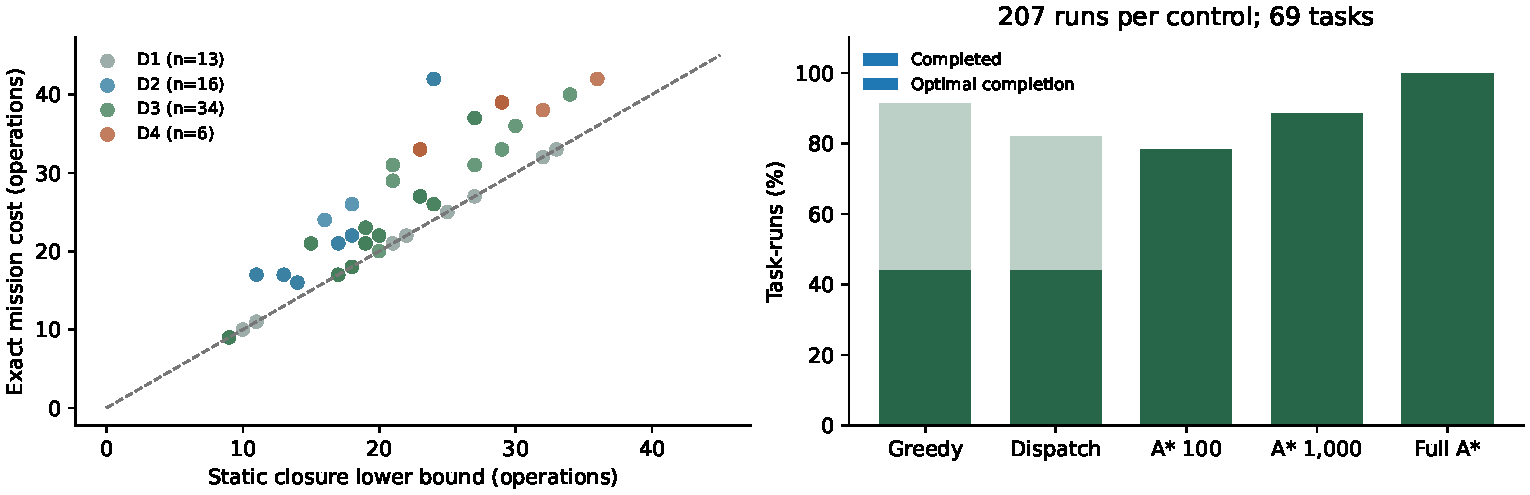
\includegraphics[width=\textwidth]{figures/mechanism-evidence.pdf}
\caption{Left: exact cost versus the strong static bound for all 69
episodes; coincident points may overlap. Right: actual completion and
optimal completion for structural controls. The tiers and tasks were
selected using mechanism and solver evidence, so these are descriptive
challenge-bank measurements.}
\end{figure*}

\section{Validation, limitations and use}
Exhaustive oracle certificates are supplemented by independent runtime
edge checks, replay of all 69 episode witnesses and 196 probe transcripts,
regret identities, overlapping recovery events, missing-assignment
censoring and tamper rejection. Ten protocol tests cover restart,
idempotence, rollback, usage accounting, study isolation and a real offline
adapter-to-HTTP-to-collection round trip. Ten Firefox checks exercise
rasters, saved views, action guards, replay, 3D review, frozen probes,
persistence and mobile layout. These checks validate software behavior;
they are not human usability or hardware construction experiments.

The upgraded bank defeats a demonstrated exact static-cost shortcut and
introduces measurable mission-state dependence, but it remains small,
public and deterministic. All states are finite and all retained legal
actions preserve solvability. Inspection is deterministic and public;
holder capacity abstracts workspace resources. We do not model free poses,
rotation, simultaneous subassembly motion, gravity, clutch forces, hand
access or rack transfer geometry. A source drawing or a collision proxy
does not validate these omitted phenomena.

The current evidence supports a reproducible research instrument and
algorithm-conditioned challenge bank. It does not establish visual-model
shortsightedness, a human--model gap, robustness to all shortcuts or
publication readiness. The next empirical requirement is a preregistered
image-versus-structured model/human study, followed by independently
acquired source families and additional mechanisms. The release preserves
earlier versions and provides its exact scope, negative findings and
reproducible artifacts so those claims can be tested.

\begin{thebibliography}{9}\small
\bibitem{ltron}
Aaron Walsman, Muru Zhang, Klemen Kotar, Karthik Desingh, Ali Farhadi,
and Dieter Fox.
Break and Make: Interactive Structural Understanding Using LEGO Bricks.
ECCV, 2022. \url{https://arxiv.org/abs/2207.13738}.
\bibitem{instructionet}
Aaron Walsman, Muru Zhang, Adam Fishman, Ali Farhadi, and Dieter Fox.
Learning to Build by Building Your Own Instructions.
2024. \url{https://arxiv.org/abs/2410.01111}.
\bibitem{astar}
Peter E. Hart, Nils J. Nilsson, and Bertram Raphael.
A Formal Basis for the Heuristic Determination of Minimum Cost Paths.
IEEE Transactions on Systems Science and Cybernetics, 4(2):100--107, 1968.
\end{thebibliography}

\clearpage
\onecolumn
\appendix
\section{Exact oracle and audit details}
\paragraph{Static audit reproducibility.}
The archived \texttt{data/predecessor-static-audit.json} contains one row
per preceding profile. The original research audit enumerates every
nonnegative label in every stored goal table, computes occupied-blocker
closure and compares Eq.~\ref{eq:old} with the label. This establishes
equality only over that finite census. It neither proves the formula exact
on arbitrary goals nor reconstructs a plan from visual observations.

\paragraph{Admissibility of the new bound.}
An initially unwanted occupied piece must be removed. A missing target
piece must be inserted, requiring removal of every occupied blocker along
its fixed insertion path. Every occupied unfinished inspection piece must
be removed to a rack holder. Each required removal recursively requires
removal of its occupied path blockers. Therefore every occupied target
piece in the resulting closure must be detached and reattached at least
once. Initially mismatched sites need at least one operation each, and
each unfinished audit costs one. These disjoint operation counts give
Eq.~\ref{eq:bound}. Connectivity and rack scheduling can add operations
but cannot invalidate the lower bound.

\paragraph{Bellman certificates.}
For a nonterminal product node $x$, the verifier checks
$C^*(x)=\min_{a\in A(x)}(1+C^*(T(x,a)))$ and $C^*(g,J)=0$.
Each physical graph edge is compared with the runtime's independent
transition enumeration, and its inverse is executed. Audit edges are
also replayed through the mission runtime. Every state in every retained
table reaches the terminal. Counts across tables repeat physical
states under different goals/job sets and must not be presented as the
number of independent tasks.

\paragraph{Why no genuine irreversible dead ends exist.}
The physical graph is reversible within its capacity-constrained component.
All admitted job pieces can be exposed in that component. Completing a job
adds a persistent bit and never removes an available physical action.
Thus any retained legal successor can still reach the goal and finish
remaining audits. A legal choice can add cost, consume scarce budget or
delay inspection, but it cannot cause permanent geometric unreachability.
This is why the unreachable-choice metric is undefined in this release.

\section{Heuristic and control diagnostics}
\begin{center}
\small\begin{tabular}{rrrrr}\toprule
Depth & Choices & All optimal & Any optimal & Uniform tie\\\midrule
1 & 98 & 49 & 98 & 74.7\%\\
2 & 98 & 61 & 98 & 78.9\%\\
4 & 98 & 49 & 98 & 70.8\%\\
8 & 98 & 66 & 98 & 81.8\%\\
\bottomrule\end{tabular}

\end{center}
The table evaluates the 98 selected next-action probes. ``All optimal''
is a pessimistic tie bound; ``Any optimal'' is the optimistic bound.
The depth-one minimum already includes an optimal action at every selected
checkpoint. Consequently, these probes do not show that shallow reasoning
must exclude the correct action. They expose ambiguity among tied choices.
Uniform tie correctness is a theoretical average over the minimizing set,
not a sampled policy run. Deeper search can change ties nonmonotonically;
the measured depth-four result is worse than depth two and is retained
without relabeling. No ``required internal lookahead depth'' is inferred.

\begin{center}
\small\begin{tabular}{lrrrr}\toprule
Control & D1 & D2 & D3 & D4\\\midrule
Closure greedy & 39/39 & 42/48 & 96/102 & 12/18\\
Capacity dispatch & 39/39 & 42/48 & 83/102 & 6/18\\
Closure A* (100) & 39/39 & 39/48 & 84/102 & 0/18\\
Closure A* (1,000) & 39/39 & 42/48 & 93/102 & 9/18\\
Closure A* (full) & 39/39 & 48/48 & 102/102 & 18/18\\
Hamming A* (full) & 39/39 & 48/48 & 102/102 & 18/18\\
\bottomrule\end{tabular}

\end{center}
Counts are task-runs, with three repeated tie-order seeds. D4 is explicitly
selected using the 100-expansion closure-A* criterion, so its zero completion
at that cap is partly a selection property. D2 can exceed D4 in search
effort. Some source groups remain easy: geometry size, tier and solution
length should not be pooled into a single unqualified hardness claim.

All raw plans, final states, node expansions, elapsed times, rejection
codes and per-run regrets are archived in
\texttt{data/software-control-records.json.gz}. Aggregates are in
\texttt{data/software-controls.json}; \texttt{controls.py} recomputes them.
The 500,000 expansion cap is an upper resource limit, not the number
of expansions consumed. Oracle table loading time is not comparable to
online A* time. Local timings share caches and lack statistical calibration.

\section{Metric denominators and event semantics}
\begin{center}\small
\begin{tabular}{p{.20\textwidth}p{.35\textwidth}p{.34\textwidth}}\toprule
Output & Denominator / eligibility & Missing and termination treatment\\\midrule
Completion & All assigned episodes & Unstarted and unfinished episodes are not successful\\
Avoidable-cost choice & Legal decisions with both zero- and positive-excess alternatives & Invalid attempts excluded; their cost remains in total excess\\
Budget-loss choice & Legal decisions with viable start budget and both viable/nonviable alternatives & Other budget losses remain in decision records\\
True unreachability & No eligible choices in retained components & Undefined, not zero evidence\\
Successful mean regret & Successfully finished episodes & Null for failures; always accompany with success coverage\\
Recovery bounds & Every legal positive-excess event & Lower: restored/all; upper adds only censored events\\
Diagnosis accuracy & Accepted diagnosis requests & Unsampled intervals are not inferred correct\\
Pair consistency & Fully assigned pairs & Missing member prevents joint credit\\
Probe correctness & All assigned probes of that kind & Missing or invalid answer gets no credit\\\bottomrule
\end{tabular}
\end{center}

\paragraph{Recovery corridor computation.}
Starting from checkpoint $b$, traverse only edges satisfying
$C^*(T(x,a))=C^*(x)-1$. The reached states are exactly
$\mathcal C_b$: every such traversal is an optimal prefix, and every state
on an optimal completion has one. Corridor membership can therefore be
checked without exploring irrelevant detours.
Each new positive-excess action starts a separate event. Later physical
steps update every active event, so a second error cannot overwrite the
first. Rejected operations consume time but cannot change corridor
membership. Terminal-unrestored events are known failures to restore;
unfinished events are censored.

\paragraph{Inspection and regret conservation.}
Successful attaches and detaches satisfy $A-D=\Delta$.
Every successful trace contains exactly $u$ accepted audits; duplicate
audits are invalid and do not change the ledger. Hence
$T=A+D+u+N_{\mathrm{invalid}}=2D+\Delta+u+N_{\mathrm{invalid}}$.
An optimal trace contains no rejection, giving
$C^*(x_0)=2D^*+\Delta+u$ and the regret identity in the main text.
Failed finish attempts and rejected camera/diagnosis requests are charged
when the runtime classifies them as invalid operation attempts.
Network-level malformed envelopes and stale revisions are rejected before
mutation and do not become action events.

\paragraph{Diagnosis and suffix reports.}
A diagnosis refers to legal avoidable-cost events since the previous
diagnosis or start, rather than whether the current assembly merely needs
rework. The first later diagnosis is attached to each previously undiagnosed
event, with its sign and attempt lag. Only true positive diagnoses open
replanning suffix records. The report retains all raw events so event
coverage, false alarms and repeated reports can be inspected separately.
An always-negative or selectively queried strategy can make aggregate
diagnosis accuracy misleading; it must be read with error-event detection.

\paragraph{Survival interpretation.}
The default curve is pooled over assigned task budgets. It is a descriptive
record with explicit denominators at each operation index, not a
Kaplan--Meier population estimate. Missing and short unfinished traces
contribute unknown outcomes; restoration never erases the first cost loss.
Compare conditions only on matched assignments and report the task/source
composition. An experiment requiring source-stratified curves should
register and report those strata before pooling.

\section{Sources, geometry and visual provenance}
\begin{center}
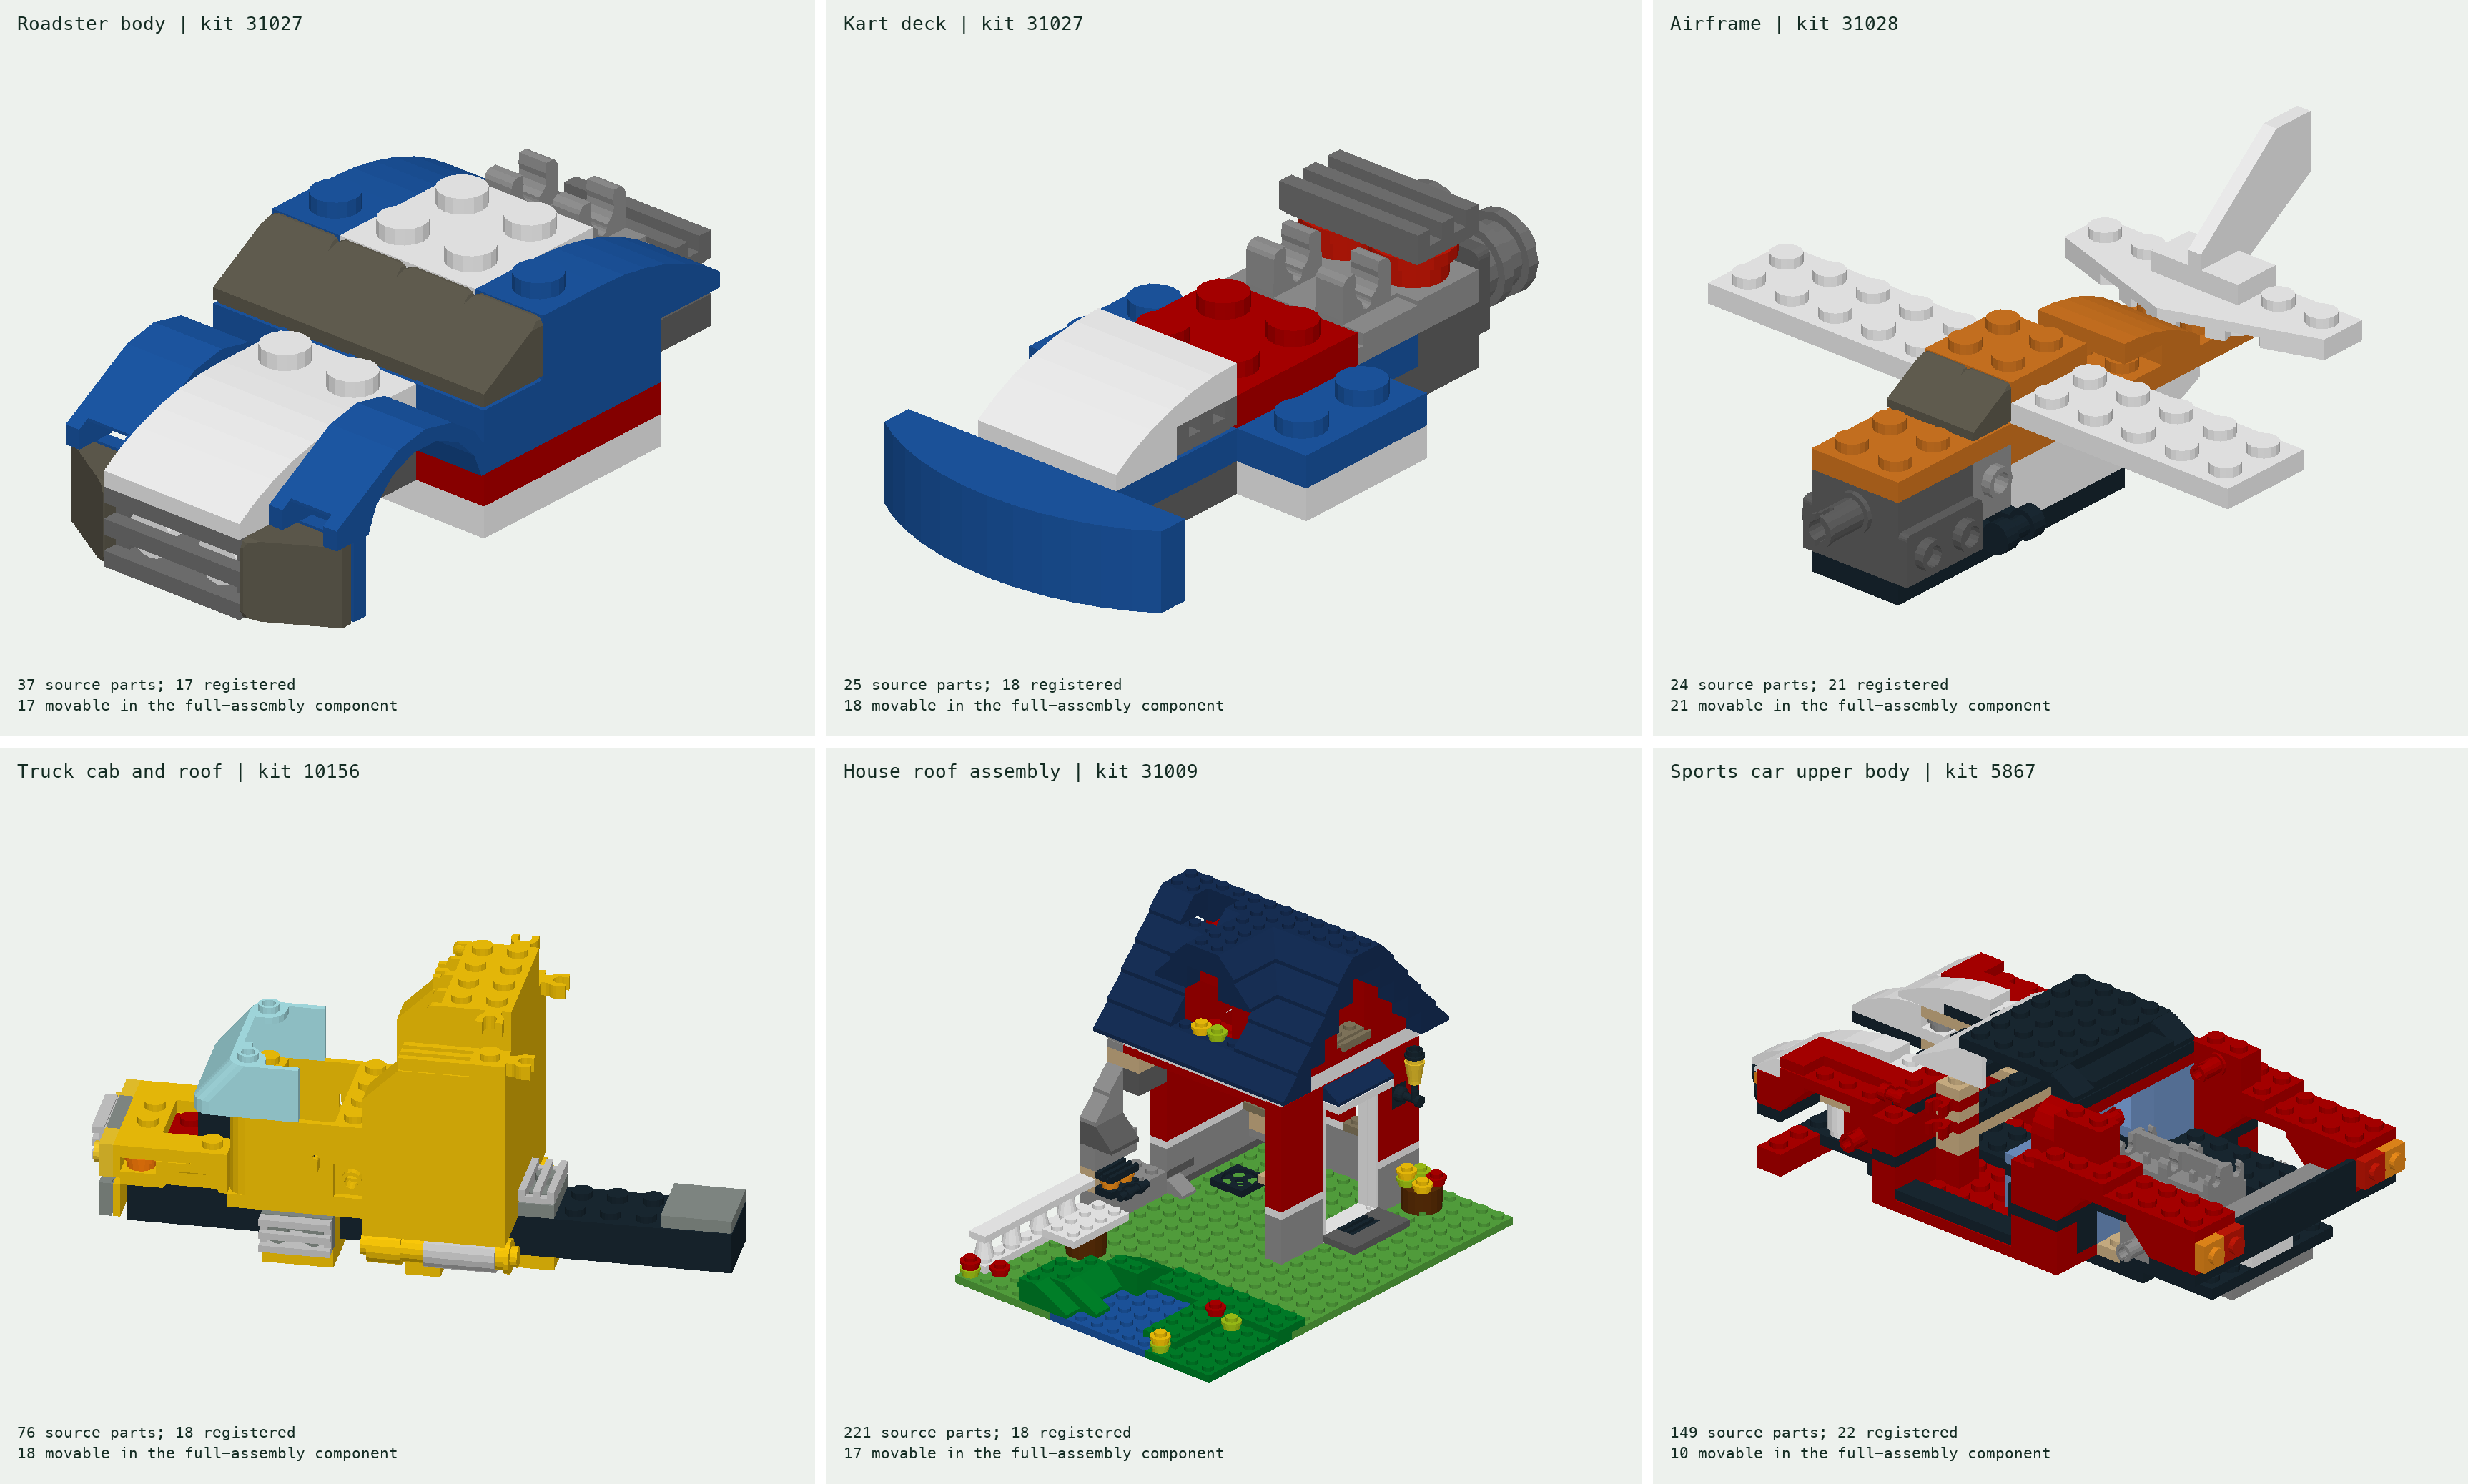
\includegraphics[width=.97\textwidth]{figures/source-gallery.png}
\end{center}
All six full source subassemblies are shown without exploded transforms.
The fixed part count can dominate the visual scene and does not increase
the number of decision variables. Roadster and kart are grouped together
by source kit. The cottage and sports car retain mechanically locked
registered sites; their active size is reported explicitly.

The flattened display atlas contains 94 distinct part meshes from 336
locked source files. \texttt{data/render-provenance.json} records every
source hash and the mesh-atlas digest. The generated figures use the
same triangle raster as the observation interface, at publication
resolution. \texttt{figures/provenance.json} binds task states, seed,
mesh digest and figure hashes. The plot uses measured task/control data.
No generated illustrative substitute meshes or model-output images are used.

Source models are attributed to Merlijn Wissink (31027 and 31028),
Robert Paciorek (10156), Stefan Frenz (31009), and Takeshi Takahashi (5867),
with the exact OMR URLs and licenses in \texttt{ASSET-LICENSES.json}.
Part-level authors and notices are preserved there separately.
The source models use CC BY 2.0; part notices identify their applicable
CC BY licenses. Original LDraw triangles, source matrices and registered
IDs remain traceable. Geometry proxies are used only for qualification,
not as substituted display shapes.

\section{Protocol, trust boundaries and acceptance evidence}
The full HTTP and external-adapter schemas are specified in
\texttt{PROTOCOL.md}. Study collections bind run, participant, condition,
seed, assignments and bank hash. An evaluator replays all mutation
requests, recomputes outcomes, verifies view histories and normalizes
permuted candidate indices before scoring. A request ID reused with
changed content or stale revision is rejected. Identical retries return
their original acknowledgment without repeating operations.

Study mode excludes score/replay/free-3D endpoints and private static
assets. Practice exposes those only for ended episodes. Neither local
files nor export digests form a cryptographic guarantee against an
administrator editing both data and code. Records must remain on the
evaluator host. The loopback server is a single-participant development
service; remote deployments require per-participant isolation and an
authenticated gateway.

The external process adapter has no built-in provider call or paid model.
Reported-usage mode reserves the declared maximum per-call input/output
tokens and currency before invocation. The adapter must account for all
images and context, enforce limits and attest that it did so.
Incomplete usage, timeout or malformed output leaves a durable failed or
unknown call and stops automatic continuation. Unknown provider usage
cannot be silently cleared by restarting. Unavailable-accounting mode
reports tokens and currency as unavailable, not as zero.
Every call has full input/output, identity and configuration hashes,
timestamps/latency, usage, request IDs and error records.

\begin{center}\small
\begin{tabular}{p{.32\textwidth}p{.55\textwidth}}\toprule
Acceptance layer & Evidence\\\midrule
Exact domain/oracle & 35 exhaustive tables; runtime edges, Bellman equalities, lower bounds and physical inverses\\
Semantic evaluation & 69 episode replays; 196 probe transcripts; cost/recovery/censoring identities and tamper rejection\\
HTTP / adapter & 10 tests covering restart, idempotence, view limits, rollback, private-route isolation, usage budgets and offline end-to-end collection\\
Browser & 10 Firefox checks; source pixels, saved views, action guards, 3D orbit/explosion, frozen probes, reload and mobile layout\\
Manuscript and release & Generated table/data consistency, figure provenance, predecessor hash audit and release manifest\\\bottomrule
\end{tabular}
\end{center}
Reference-action software acceptance is not participant performance.
Browser screenshots and test outputs are archived under
\texttt{tem/brickplan-v2/validation/}. The current manuscript uses a
generic two-column research layout; conference-template formatting,
full contemporary related-work coverage and empirical model/human
results remain submission work.

\section{Complete episode census}
``Jobs'' is the total declared inspection count, ``Done'' is its initially
completed subset, and A* expansions use seed 0 and the closure heuristic.
Internal IDs below are evaluator documentation; participant catalogs use
opaque identifiers. Exact start/goal masks, ordered jobs, optimal actions,
witnesses and oracle paths are in the private task bank.
\small
\begin{longtable}{llrrrrrr}
\toprule Episode & Tier & Rack & Jobs & Done & $C^*$ & $h$ & A* exp.\\\midrule\endhead
roadster-body-01 & D1 & 17 & 0 & 0 & 17 & 17 & 17\\
roadster-body-02 & D1 & 17 & 0 & 0 & 32 & 32 & 32\\
roadster-body-03 & D2 & 9 & 0 & 0 & 27 & 23 & 33\\
roadster-body-04 & D2 & 9 & 0 & 0 & 27 & 23 & 38\\
roadster-body-05 & D2 & 9 & 0 & 0 & 42 & 24 & 2555\\
roadster-body-06 & D2 & 9 & 0 & 0 & 42 & 24 & 2555\\
roadster-body-07 & D3 & 9 & 2 & 0 & 37 & 27 & 2185\\
roadster-body-08 & D3 & 9 & 2 & 0 & 37 & 27 & 2139\\
roadster-body-09 & D3 & 9 & 2 & 1 & 20 & 20 & 21\\
roadster-body-10 & D3 & 9 & 2 & 1 & 18 & 18 & 18\\
roadster-body-11 & D3 & 9 & 1 & 0 & 18 & 18 & 18\\
roadster-body-12 & D3 & 9 & 1 & 0 & 18 & 18 & 18\\
roadster-body-13 & D4 & 9 & 4 & 0 & 39 & 29 & 2131\\
roadster-body-14 & D4 & 9 & 4 & 0 & 39 & 29 & 2129\\
kart-deck-01 & D1 & 18 & 0 & 0 & 18 & 18 & 18\\
kart-deck-02 & D1 & 18 & 0 & 0 & 25 & 25 & 25\\
kart-deck-03 & D2 & 5 & 0 & 0 & 17 & 11 & 32\\
kart-deck-04 & D2 & 5 & 0 & 0 & 17 & 11 & 32\\
kart-deck-05 & D2 & 5 & 0 & 0 & 26 & 18 & 119\\
kart-deck-06 & D2 & 5 & 0 & 0 & 24 & 16 & 90\\
kart-deck-07 & D3 & 5 & 2 & 0 & 31 & 21 & 121\\
kart-deck-08 & D3 & 5 & 2 & 0 & 29 & 21 & 218\\
kart-deck-09 & D3 & 5 & 2 & 1 & 21 & 15 & 68\\
kart-deck-10 & D3 & 5 & 2 & 1 & 23 & 19 & 42\\
kart-deck-11 & D3 & 5 & 1 & 0 & 23 & 19 & 42\\
kart-deck-12 & D3 & 5 & 1 & 0 & 21 & 15 & 68\\
kart-deck-13 & D4 & 5 & 4 & 0 & 33 & 23 & 403\\
kart-deck-14 & D4 & 5 & 4 & 0 & 33 & 23 & 392\\
airframe-01 & D1 & 21 & 0 & 0 & 21 & 21 & 21\\
airframe-02 & D1 & 21 & 0 & 0 & 33 & 33 & 33\\
airframe-03 & D2 & 8 & 0 & 0 & 16 & 14 & 16\\
airframe-04 & D2 & 8 & 0 & 0 & 16 & 14 & 16\\
airframe-05 & D2 & 8 & 0 & 0 & 17 & 13 & 30\\
airframe-06 & D2 & 8 & 0 & 0 & 17 & 13 & 30\\
airframe-07 & D3 & 8 & 2 & 0 & 22 & 20 & 22\\
airframe-08 & D3 & 8 & 2 & 0 & 22 & 20 & 22\\
airframe-09 & D3 & 8 & 2 & 1 & 9 & 9 & 9\\
airframe-10 & D3 & 8 & 2 & 1 & 9 & 9 & 9\\
airframe-11 & D3 & 8 & 1 & 0 & 9 & 9 & 9\\
airframe-12 & D3 & 8 & 1 & 0 & 9 & 9 & 9\\
airframe-13 & D3 & 8 & 4 & 0 & 26 & 24 & 26\\
airframe-14 & D3 & 8 & 4 & 0 & 26 & 24 & 26\\
truck-cab-01 & D1 & 18 & 0 & 0 & 18 & 18 & 18\\
truck-cab-02 & D1 & 18 & 0 & 0 & 27 & 27 & 27\\
truck-cab-03 & D3 & 12 & 2 & 0 & 40 & 34 & 1522\\
truck-cab-04 & D3 & 12 & 2 & 0 & 36 & 30 & 809\\
truck-cab-05 & D3 & 12 & 2 & 1 & 21 & 19 & 22\\
truck-cab-06 & D3 & 12 & 2 & 1 & 21 & 19 & 22\\
truck-cab-07 & D3 & 12 & 1 & 0 & 21 & 19 & 22\\
truck-cab-08 & D3 & 12 & 1 & 0 & 21 & 19 & 22\\
truck-cab-09 & D4 & 12 & 4 & 0 & 42 & 36 & 1546\\
truck-cab-10 & D4 & 12 & 4 & 0 & 38 & 32 & 831\\
house-roof-01 & D1 & 18 & 0 & 0 & 18 & 18 & 18\\
house-roof-02 & D1 & 18 & 0 & 0 & 22 & 22 & 22\\
house-roof-03 & D2 & 5 & 0 & 0 & 21 & 17 & 37\\
house-roof-04 & D2 & 5 & 0 & 0 & 21 & 17 & 37\\
house-roof-05 & D2 & 5 & 0 & 0 & 22 & 18 & 45\\
house-roof-06 & D2 & 5 & 0 & 0 & 22 & 18 & 45\\
house-roof-07 & D3 & 5 & 2 & 0 & 27 & 23 & 54\\
house-roof-08 & D3 & 5 & 2 & 0 & 27 & 23 & 50\\
house-roof-09 & D3 & 5 & 2 & 1 & 17 & 17 & 19\\
house-roof-10 & D3 & 5 & 2 & 1 & 17 & 17 & 23\\
house-roof-11 & D3 & 5 & 1 & 0 & 17 & 17 & 23\\
house-roof-12 & D3 & 5 & 1 & 0 & 17 & 17 & 19\\
house-roof-13 & D3 & 5 & 4 & 0 & 33 & 29 & 76\\
house-roof-14 & D3 & 5 & 4 & 0 & 31 & 27 & 68\\
sports-body-01 & D1 & 22 & 0 & 0 & 10 & 10 & 10\\
sports-body-02 & D1 & 22 & 0 & 0 & 11 & 11 & 11\\
sports-body-03 & D1 & 8 & 2 & 0 & 17 & 17 & 17\\
\bottomrule\end{longtable}

\normalsize

\end{document}
